\documentclass[tikz]{standalone}
\usetikzlibrary{intersections}
\begin{document}
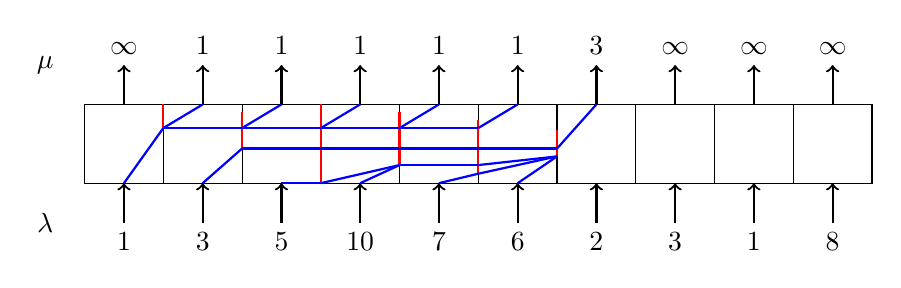
\begin{tikzpicture}
  % \useasboundingbox (0,3.5) rectangle (6,-0.5);

  \foreach \i/\l/\m in {1/1/\infty, 2/3/1, 3/5/1, 4/10/1, 5/7/1, 6/6/1, 7/2/3, 8/3/\infty, 9/1/\infty, 10/8/\infty}{
    \pgfmathsetmacro{\prev}{\i-1}
    \pgfmathsetmacro{\mid}{\i-0.5}
		\draw (\prev, 0) rectangle (\i, 1);
		\draw[->, thick] (\mid,-0.5) -- (\mid,0) node[pos=0,below] {\(\l\)};
		\draw[->, thick] (\mid,1) -- (\mid,1.5) node[pos=1,above] {\(\m\)};
  }

	\foreach \i/\a/\b in {1/0.7/1, 2/0.44/0.9, 3/0/1, 4/0.23/0.9, 5/0.12/0.8, 6/0.34/0.68}{
		\draw[color=red, thick] (\i, \a) -- (\i, \b);
	}
	\node at (-0.5,-0.5) {\(\lambda\)};
	\node at (-0.5,1.5) {\(\mu\)};
	\draw[color=blue, thick] (0.5,0) -- (1,0.7);
	\draw[color=blue, thick] (1,0.7) -- (2,0.7);
	\draw[color=blue, thick] (1,0.7) -- (1.5,1);
	\draw[color=blue, thick] (2,0.7) -- (3,0.7);
	\draw[color=blue, thick] (2,0.7) -- (2.5,1);
	\draw[color=blue, thick] (3,0.7) -- (4,0.7);
	\draw[color=blue, thick] (3,0.7) -- (3.5,1);
	\draw[color=blue, thick] (4,0.7) -- (5,0.7);
	\draw[color=blue, thick] (4,0.7) -- (4.5,1);
	\draw[color=blue, thick] (5,0.7) -- (5.5,1);

	\draw[color=blue, thick] (1.5,0) -- (2,0.44);
	\draw[color=blue, thick] (2,0.44) -- (3,0.44);
	\draw[color=blue, thick] (3,0.44) -- (4,0.44);
	\draw[color=blue, thick] (4,0.44) -- (5,0.44);
	\draw[color=blue, thick] (5,0.44) -- (6,0.44);
	\draw[color=blue, thick] (6,0.44) -- (6.5,1);


	\draw[color=blue, thick] (2.5,0) -- (3,0);
	\draw[color=blue, thick] (3,0) -- (4,0.23);
	\draw[color=blue, thick] (3.5,0) -- (4,0.23);
	\draw[color=blue, thick] (4,0.23) -- (5,0.23);
	\draw[color=blue, thick] (4.5,0) -- (5,0.12);
	\draw[color=blue, thick] (5,0.12) -- (6,0.34);
	\draw[color=blue, thick] (5.5,0) -- (6,0.34);
	\draw[color=blue, thick] (5,0.23) -- (6,0.34);
\end{tikzpicture}
\end{document}
